Sekvens is an application that allows guardians to present sequences of pictograms to autistic children. This aids the autistic children in performing daily routines, which they would not be capable of without a visualization. Examples of sequences could be a sequence for how to wash hands, how to put on outdoor clothing during winter, or how to behave during dinner. Sekvens is a digital solution to an existing analog solution which is currently used in institutions in and near the city of Aalborg.

\begin{figure} [h!]
\centering
\begin{minipage}{.7\textwidth}
\centering
\fbox{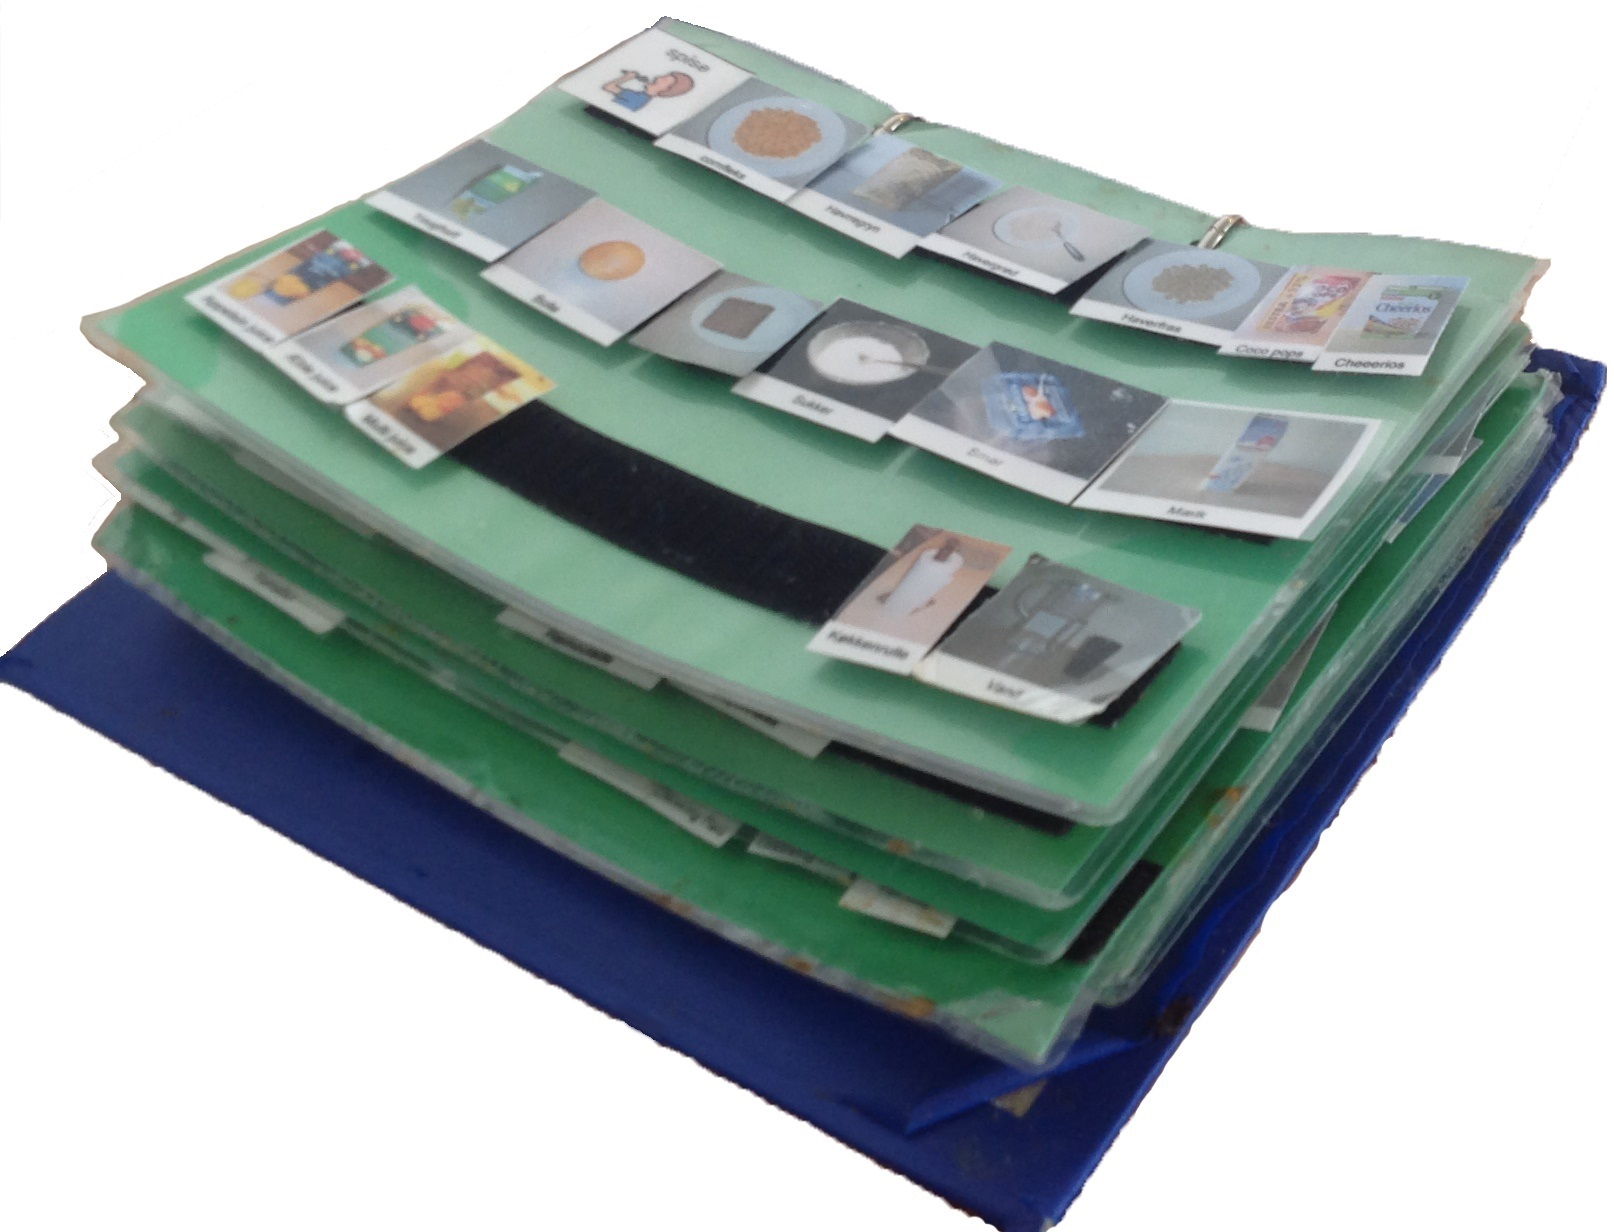
\includegraphics[scale=0.17]{Pics/Sprint1/pictogram_binder.jpg}}
\caption{A pictogram binder with already constructed sequences}
\label{fig:pictogram_binder}
\fbox{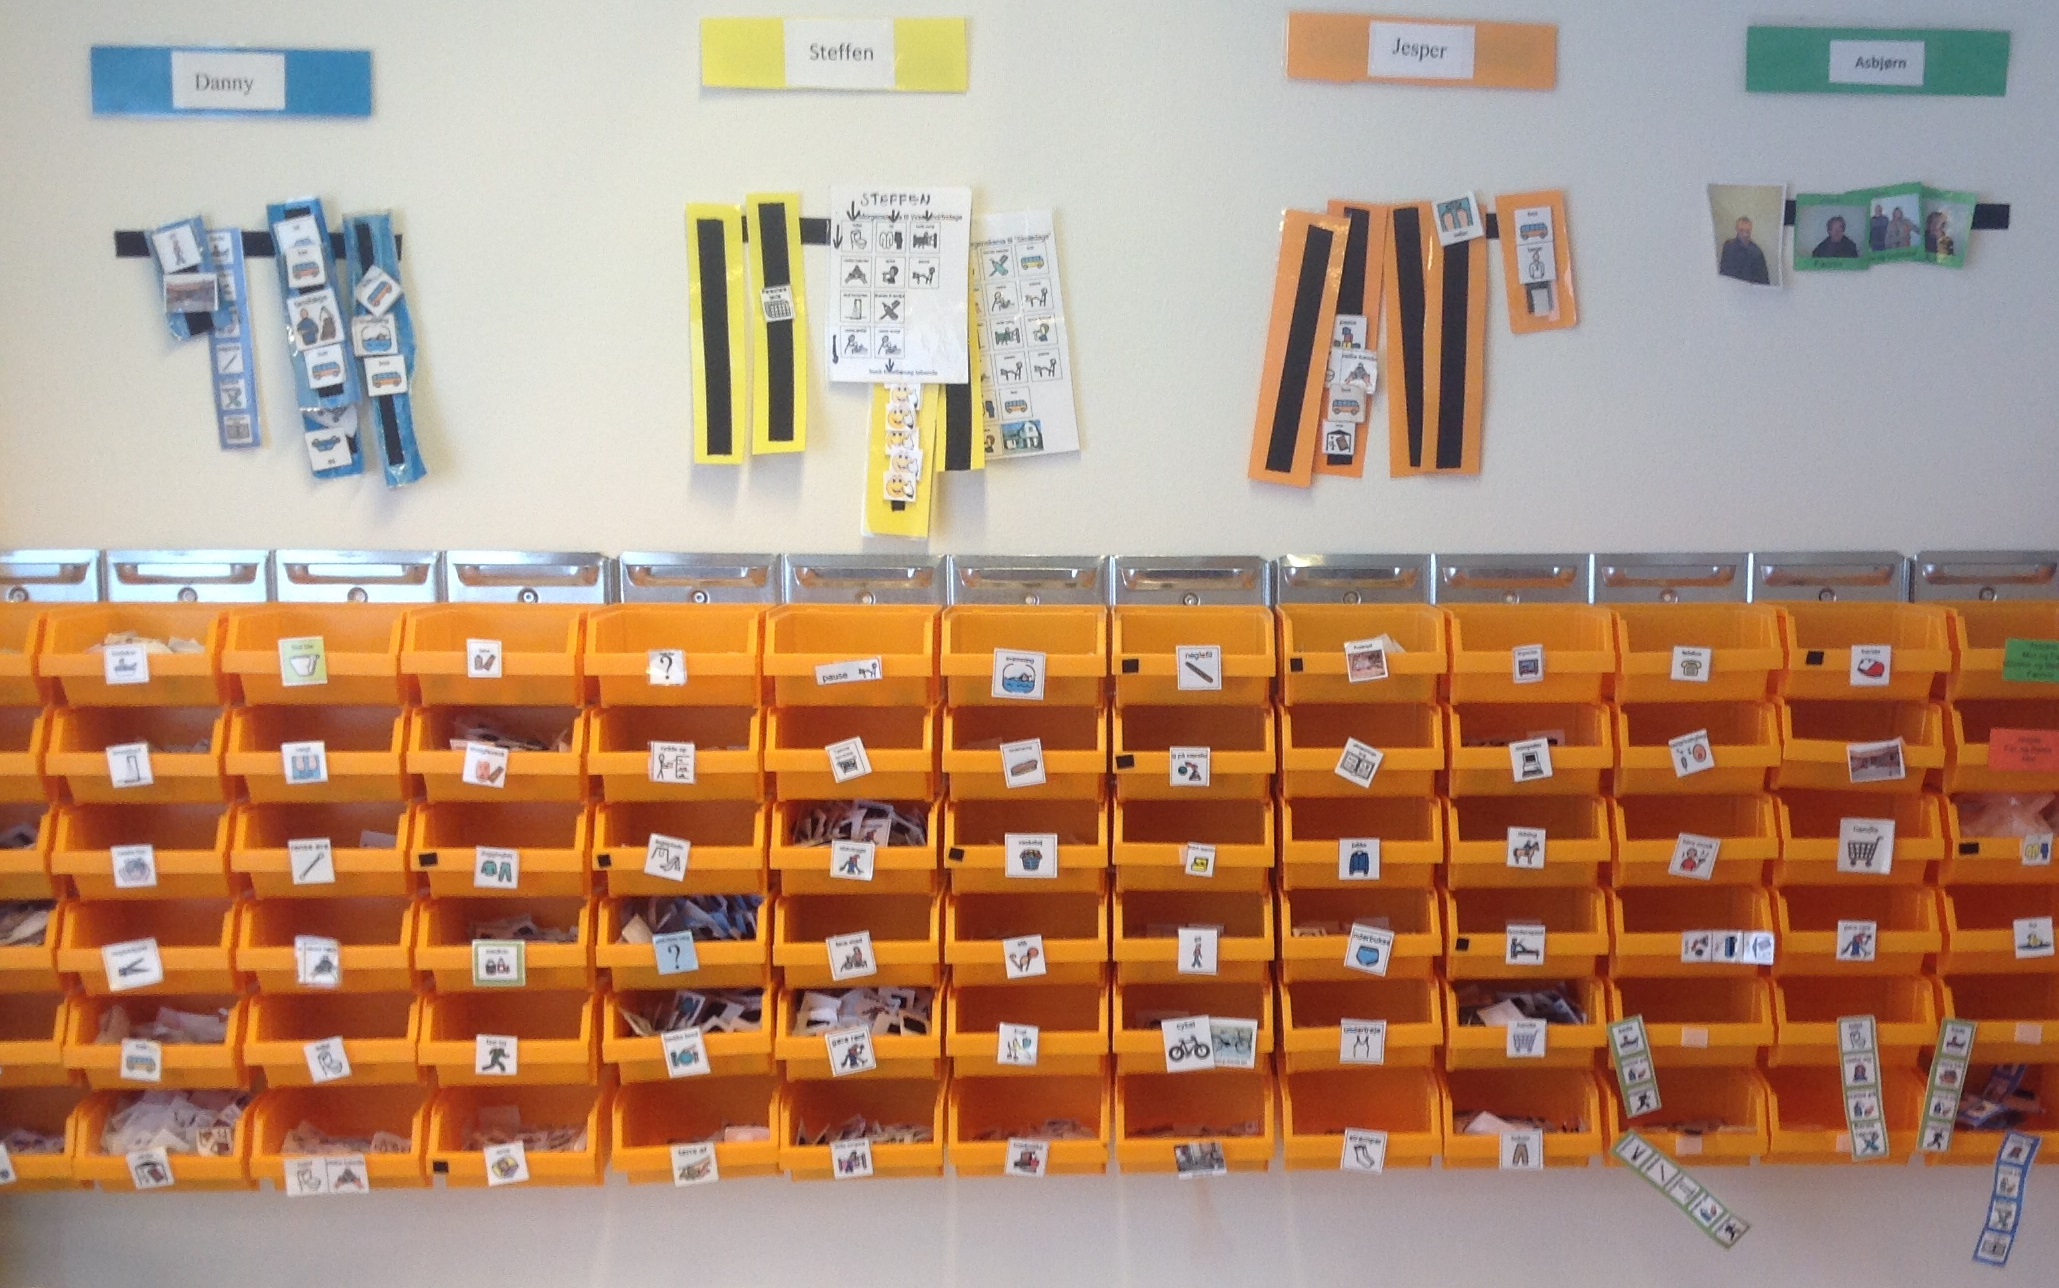
\includegraphics[scale=0.14]{Pics/Sprint1/pictogram_containers.jpg}}
\caption{Pictogram containers and personal sequences for the children}
\label{fig:pictogram_container}
\end{minipage}\hfill
\begin{minipage}{.3\textwidth}
\centering
\fbox{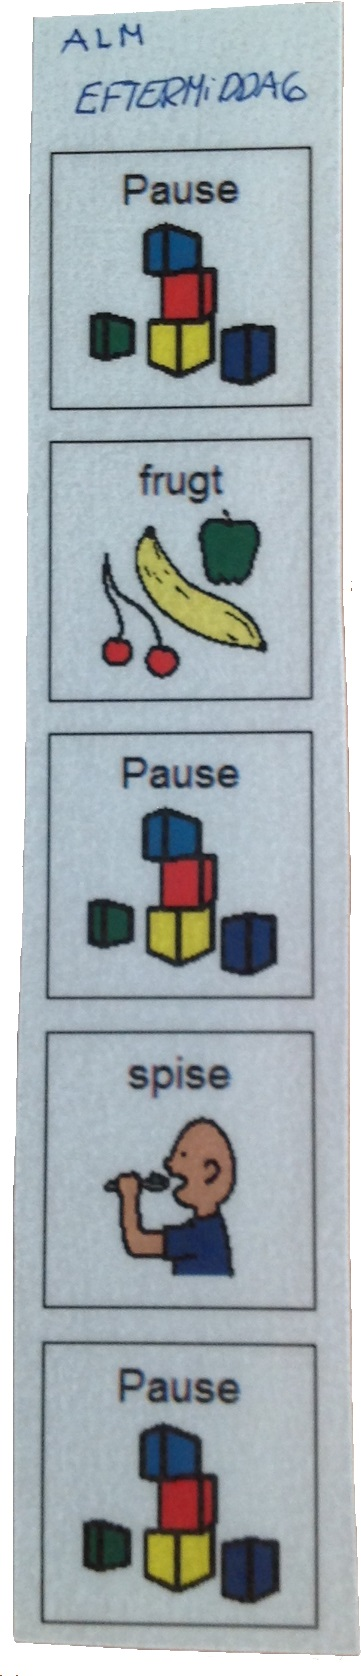
\includegraphics[scale=0.17]{Pics/Sprint1/pictogram_sequence.jpg}}
\caption{A sequence of pictograms made for eating an afternoon meal}
\label{fig:sequence}
\end{minipage}
\end{figure}

It is quite obvious, that the current solution is exhaustive (An example of a current solution is portrayed in figure \ref{fig:pictogram_binder},\ref{fig:pictogram_container} and \ref{fig:sequence} ). It was previously decided by a group of software students on 6th semester, to work on a digital solution. They created a first draft of the application that we picked up. They had a standalone application running, but had remaining issues and obstacles they did not have time to solve.

During sprint 1, our goal was to solve the remaining issues and obstacles for the application rather than developing new features or creating additional functionality for already existing features. This was a common agreement among the software 6 students working on the GIRAF multi-project.




